\documentclass[a4paper,12pt]{article}

\usepackage[utf8]{inputenc}
\usepackage[T1]{polski}
\usepackage{helvet}
\usepackage{graphicx}
\usepackage{color}
\usepackage{xcolor}
\usepackage{geometry}
\usepackage{caption}
\usepackage{makeidx}
\usepackage{wrapfig}
\usepackage{listings}


\geometry{hmargin={2cm, 2cm}, height=10.0in}
\DeclareCaptionFont{white}{\color{white}}
\DeclareCaptionFormat{listing}{\colorbox{gray}{\parbox{\textwidth}{#1#2#3}}}
\captionsetup[lstlisting]{format=listing,labelfont=white,textfont=white}
\lstset{ %
language=Octave,                % choose the language of the code
basicstyle=\footnotesize,       % the size of the fonts that are used for the code
numbers=left,                   % where to put the line-numbers
numberstyle=\footnotesize,      % the size of the fonts that are used for the line-numbers
stepnumber=1,                   % the step between two line-numbers. If it's 1 each line 
                                % will be numbered
numbersep=5pt,                  % how far the line-numbers are from the code
backgroundcolor=\color{white},  % choose the background color. You must add \usepackage{color}
showspaces=false,               % show spaces adding particular underscores
showstringspaces=false,         % underline spaces within strings
showtabs=false,                 % show tabs within strings adding particular underscores
frame=single,	                % adds a frame around the code
tabsize=2,	                % sets default tabsize to 2 spaces
%captionpos=b,                   % sets the caption-position to bottom
breaklines=true,                % sets automatic line breaking
breakatwhitespace=false,        % sets if automatic breaks should only happen at whitespace
title=\lstname,                 % show the filename of files included with \lstinputlisting;
                                % also try caption instead of title
escapeinside={\%*}{*)},         % if you want to add a comment within your code
morekeywords={*,...}            % if you want to add more keywords to the set
}

\lstloadlanguages{ Ruby }


\makeindex

\begin{document}

% =====  STRONA TYTULOWA PRACY INŻYNIERSKIEJ ====
% ostatnia modyfikacja: 2009/07/01, K. Malarz

\thispagestyle{empty}

%% ------------------------ NAGLOWEK STRONY ---------------------------------
\begin{figure}
\vspace{-13cm}
\hspace{-4cm}

\includegraphics[height=29.3cm]{agh_nzw_a_pl_1w_wbr_cmyk.pdf}\\
\vspace{-13.9cm}
\end{figure}
\rule{26mm}{0pt}
{\large\textsf{Wydział Fizyki i Informatyki Stosowanej}}\\
\rule{\textwidth}{3pt}\\
\rule[2ex]
{\textwidth}{1pt}\\
\vspace{7ex}
\begin{center}
{\bf\LARGE\textsf{Analiza i przetwarzanie obrazów}}\\
\vspace{13ex}
{\bf\huge\textsf{Ćwiczenie 3}}\\
\vspace{3ex}
{\sf \small } {\bf\small\textsf{Krystian Wojtas}}\\
\vspace{14ex}
%% ------------------------ OPIEKUN PRACY ------------------------------------
{\sf \Large } {\bf\Large\textsf{}}\\
\vspace{22ex}
\textsf{\bf\large\textsf{Kraków, listopad 2011}}
\end{center}
%% =====  STRONA TYTUŁOWA PRACY INŻYNIERSKIEJ  ====


\newpage
\section{Wstęp}
Celem ćwiczeń była zmiana jasności i konrastu obrazu, zastosowanie filtrów wykrywania krawędzi - krzyż Robertsa oraz filtr Sobela, a także obrót o zadany kąt. Wykorzystany został język Ruby i jego framework RMagic, który binduje funkcje biblioteczne z pakietu ImageMagick.

\begin{figure}[h!]
   \centering
   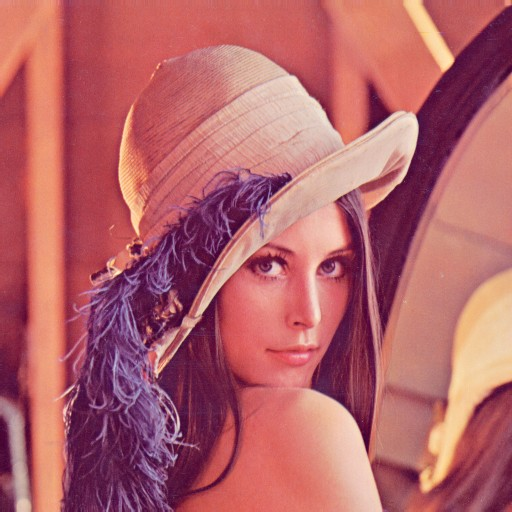
\includegraphics[width=15cm]{../out/lena.jpg}
   \caption{Obraz wzorcowy}
\end{figure}


\newpage
\section{Jasność}
Aby zmienić jasność pikseli, zastosowany został wzór
$$p(x, y) = p(x, y) + w$$
gdzie $w$ jest wartością o jaką przesuwamy barwy w poszczególnych kanałach.

\lstinputlisting[caption=Implementacja zmiany jasnosci]{listingi/jasnosc.rb}

\begin{figure}[h!]
\begin{minipage}[t]{5cm}
\begin{center}
\includegraphics[width=5cm,clip]{../out/jasnosc01q.jpg}
\caption{przesuniecie 0.1 Q}
\end{center}
\end{minipage}
\hfill
\begin{minipage}[t]{5cm}
\begin{center}
\includegraphics[width=5cm,clip]{../out/jasnosc03q.jpg}
\caption{przesuniecie 0.3 Q}
\end{center}
\end{minipage}
\hfill
\begin{minipage}[t]{5cm}
\begin{center}
\includegraphics[width=5cm,clip]{../out/jasnosc06q.jpg}
\caption{przesuniecie 0.6 Q}
\end{center}
\end{minipage}
\end{figure}

\begin{figure}[h!]
\begin{minipage}[t]{5cm}
\begin{center}
\includegraphics[width=5cm,clip]{../out/jasnoscm01q.jpg}
\caption{przesuniecie -0.1 Q}
\end{center}
\end{minipage}
\hfill
\begin{minipage}[t]{5cm}
\begin{center}
\includegraphics[width=5cm,clip]{../out/jasnoscm03q.jpg}
\caption{przesuniecie -0.3 Q}
\end{center}
\end{minipage}
\hfill
\begin{minipage}[t]{5cm}
\begin{center}
\includegraphics[width=5cm,clip]{../out/jasnoscm06q.jpg}
\caption{przesuniecie -0.6 Q}
\end{center}
\end{minipage}
\end{figure}



\newpage
\section{Kontrast}
Aby zmienić kontrast pikseli, zastosowany został wzór
$$p(x, y) = p(x, y) * w$$
gdzie $w$ jest wartością o jaką skalujemy barwy w poszczególnych kanałach.

\lstinputlisting[caption=Implementacja zmiany kontrastu]{listingi/kontrast.rb}

\begin{figure}[h!]
\begin{minipage}[t]{5cm}
\begin{center}
\includegraphics[width=5cm,clip]{../out/kontrast09.jpg}
\caption{kontrast 0.9}
\end{center}
\end{minipage}
\hfill
\begin{minipage}[t]{5cm}
\begin{center}
\includegraphics[width=5cm,clip]{../out/kontrast07.jpg}
\caption{kontrast 0.7}
\end{center}
\end{minipage}
\hfill
\begin{minipage}[t]{5cm}
\begin{center}
\includegraphics[width=5cm,clip]{../out/kontrast03.jpg}
\caption{kontrast 0.3}
\end{center}
\end{minipage}
\end{figure}

\begin{figure}[h!]
\begin{minipage}[t]{5cm}
\begin{center}
\includegraphics[width=5cm,clip]{../out/kontrast11.jpg}
\caption{kontrast 1.1}
\end{center}
\end{minipage}
\hfill
\begin{minipage}[t]{5cm}
\begin{center}
\includegraphics[width=5cm,clip]{../out/kontrast15.jpg}
\caption{kontrast 1.5}
\end{center}
\end{minipage}
\hfill
\begin{minipage}[t]{5cm}
\begin{center}
\includegraphics[width=5cm,clip]{../out/kontrast21.jpg}
\caption{kontrast 2.1}
\end{center}
\end{minipage}
\end{figure}



\newpage
\section{Krzyż Robertsa}
Filtr znajduje krawędzie na obrazie. Działa według wzoru
$$p(x,y) = |p(x,y)-p(x+1,y+1)| + |p(x+1,y)-p(x,y+1)|$$

\lstinputlisting[caption=Implementacja krzyza Robertsa]{listingi/krzyz.rb}

\begin{figure}[h!]
   \centering
   \includegraphics[width=15cm]{../out/krzyz.jpg}
   \caption{Zastosowany krzyz Robertsa}
\end{figure}



\newpage
\section{Filtr Sobela}
Filtr również znajduje krawędzie na obrazie. Dla tak nazwanych pikseli otaczających piksel środkowy $px$
\begin{center}
\[ \left( \begin{array}{ccc}
p0 & p1 & p2 \\
p7 & px & p3 \\
p6 & p5 & p4 \end{array} \right)\] 
\end{center}
zastosowanie mają wzory wyliczające nową wartość środkowego piksela
$$x = (p2+2*p3+p4)-(p0+2*p7+p6)$$
$$y = (p6+2*p5+p4)-(p0+2*p1+p2)$$
$$px = \sqrt{x^2 + y^2}$$

\lstinputlisting[caption=Implementacja filtru Sobela]{listingi/sobel.rb}

\begin{figure}[h!]
   \centering
   \includegraphics[width=15cm]{../out/sobel.jpg}
   \caption{Zastosowany filtr Sobela}
\end{figure}



\newpage
\section{Obrót}
Przed przystąpieniem do obracania obrazka, należy ustalić punkty w które trafiłyby jego rogi. Wypadną one poza ramy obrazka - to nasuwa informację o korygowanym przesunięciu oraz nowych rozmiarach.
Obrót obrazka uzyskujemy przekształcając położenie jego pikseli według wzorów na obrót punktu
$$x' = cos(r)*(x+p) - sin(r)*(y+q)$$
$$y' = sin(r)*(x+p) + cos(r)*(y+q)$$
$$p'(x,y) = p(x', y')$$
gdzie $p$ i $q$ to położenie lewego górnego rogu po obrocie oraz wektor przesunięcia wszystkich pikseli. Dzięki temu zaczynają się od (0,0).

\newpage
\lstinputlisting[caption=Implementacja obrotu]{listingi/obrot.rb}

\newpage
\begin{figure}[h!]
\begin{minipage}[t]{5cm}
\begin{center}
\includegraphics[width=5cm,clip]{../out/obrot025.jpg}
\caption{obrot 0.25 Pi}
\end{center}
\end{minipage}
\hfill
\begin{minipage}[t]{5cm}
\begin{center}
\includegraphics[width=5cm,clip]{../out/obrot01.jpg}
\caption{obrot 1.5 Pi}
\end{center}
\end{minipage}
\hfill
\begin{minipage}[t]{5cm}
\begin{center}
\includegraphics[width=5cm,clip]{../out/obrot05.jpg}
\caption{obrot 2.1 Pi }
\end{center}
\end{minipage}
\end{figure}

\begin{figure}[h!]
\begin{minipage}[t]{5cm}
\begin{center}
\includegraphics[width=5cm,clip]{../out/obrot08.jpg}
\caption{obrot 0.8 Pi}
\end{center}
\end{minipage}
\hfill
\begin{minipage}[t]{5cm}
\begin{center}
\includegraphics[width=5cm,clip]{../out/obrotm03.jpg}
\caption{obrot -0.3 Pi}
\end{center}
\end{minipage}
\hfill
\begin{minipage}[t]{5cm}
\begin{center}
\includegraphics[width=5cm,clip]{../out/obrot1.jpg}
\caption{obrot Pi}
\end{center}
\end{minipage}
\end{figure}

Obraz obrócony o kąt nie będący wielokrotnością pi/2 jest rozmiarowo większy. Zawiera więc więcej pikseli niż orginał. Puste przestrzenie uzupełniłem czernią.

\end{document}
